\documentclass{article}
\usepackage{graphicx}
\usepackage{amsmath}
\usepackage[brazilian]{babel}
\usepackage{amsthm}
\usepackage{hyperref}
\usepackage{xcolor}
\usepackage{subcaption}
\usepackage{placeins}

\renewcommand{\refname}{Referências}

\theoremstyle{definition}
\newtheorem{definition}{Definição}[section]

% Custom commmands
\newcommand\norm[1]{\left\lVert#1\right\rVert}

\def \quantity#1#2#3{\vec{#1}_{#2}^{#3}}
\def \quantitysc#1#2#3{{#1}_{#2}^{#3}}
\def \quantityg#1#2#3#4#5{\vec{#1}_{#2, #3}^{#4, #5}}
\def \quantitygsc#1#2#3#4#5{{#1}_{#2, #3}^{#4, #5}}
\def \pos#1#2{\quantity{r}{#1}{#2}}
\def \desloc#1#2{\quantity{d}{#1}{#2}}
\def \deslocsc#1#2{\quantitysc{d}{#1}{#2}}
\def \deslocg#1#2#3#4{\quantityg{d}{#1}{#2}{#3}{#4}}
\def \deslocgsc#1#2#3#4{\quantitygsc{d}{#1}{#2}{#3}{#4}}

\def \case#1#2#3{A{#1}-D{#2}-T{#3}}

\title{Simulação da Reologia e dos Padrões de Movimento de Tecidos Celulares com Anéis Ativos}
\author{Marcos Pasa e Leonardo Brunnet}

\begin{document}

\maketitle

\section{Introdução}
\paragraph{}
Cicatrização de feridas, morfogênese e evolução tumoral são processos essenciais nos organismos vivos e motivam a pesquisa de fenômenos relacionados à organização multicelular. Em particular é importante entender características físicas tais como viscosidade, plasticidade e elasticidade associadas a trocas de posições das células. Embora a genética subjacente determine as mudanças das interações microscópicas, ao final serão as características físicas que estarão em jogo na organização. Defeitos topológicos associados à ordem nemática, invaginações devido a contrações do córtex de membranas sendo  exemplos característicos. Modelos computacionais de sistemas multicelulares são ferramentas robustas para testar hipóteses e ganhar conhecimento sobre tais sistemas.

Diversos modelos de células ativas já foram desenvolvidos, sendo os mais simples aqueles que utilizam apenas o centro da célula como grau de liberdade. Nesses casos, as células podem ser representadas como esferas com volume de exclusão (\cite{vicsek_novel_1995}, \cite{gregoire_moving_2003}, \cite{szabo_phase_2006}, \cite{belmonte_self-propelled_2008}) ou como polígonos de uma tesselação de Voronoi (\cite{barton_active_2017}, \cite{bi_motility-driven_2016}). A principal vantagem desses modelos é sua simplicidade e eficiência computacional. No entanto, eles se tornam inadequados para descrever situações mais complexas. Para maior sofisticação, há modelos em que o grau de liberdade corresponde ao contorno da célula. Nesse caso, as células podem ser representadas por pixels, simulando imagens experimentais (como no modelo celular de Potts) (\cite{kabla_collective_2012}, \cite{kafer_moving_2006}), pelos vértices de polígonos que ladrilham o espaço \cite{perez-verdugo_vertex_2020} ou até mesmo por meio de um campo de fases contínuo \cite{loewe_solid-liquid_2020}.

O presente trabalho tem por objetivo implementar e explorar um modelo teórico-computacional para células biológicas em duas dimensões que inclui o contorno das células. Diferentemente de modelos mais simples, onde a distância entre os centros das células é o principal parâmetro relevante, neste caso as células são descritas como membranas compostas por partículas puntiformes conectadas por molas. Essa abordagem aumenta significativamente o número de graus de liberdade, permitindo modelar deformações da forma celular e interações mais detalhadas. Foi escolhido o modelo apresentado por Teixeira \textit{et al}. (\cite{teixeira_single_2021}, \cite{teixeira_segregation_2024}), no qual as células são representadas por polígonos cujos vértices são partículas ativas com volume de exclusão e mecanismo de autoalinhamento. As células são livres para se mover e podem interagir par a par. Além disso, o modelo incorpora a polarização associada ao centro da célula, que desempenha um papel crucial nos processos de organização e movimento celular \cite{glazenburg_polarization_2023}.

% O presente trabalho tem por objetivo implementar e explorar um modelo teórico-computacional para células biológicas com grau de liberdade no contorno das mesmas. Foi escolhido o modelo apresentado por Teixeira \textit{et al}.(\cite{teixeira_single_2021}, \cite{teixeira_segregation_2024}), em que células são representadas por polígonos cujos vértices são partículas ativas com volume de exclusão e mecanismo de auto-alinhamento. As partículas são conectadas por molas, assim possibilitando a deformação do formato das células.

Para estudar o modelo, simulamos um fluxo de células confinado em um corredor com um obstáculo circular no centro (fluxo em geometria de Stokes). Essa geometria favorece o cisalhamento e o fluxo viscoso, o que é essencial para a compreensão da deformação heterogênea e taxa de rearranjo das células. Experimentos com células em geometria de Stokes é viável e já foi realizado diversas vezes (\cite{kim_propulsion_2013}, \cite{duran_2020}). 
Seguimos no mesmo espirito no trabalho feito por Beatrici \textit{et al}. \cite{beatrici_comparing_2023}, em que 5 modelos de células móveis foram comparados no fluxo de Stokes. Escolhemos 3 parâmetros para variar durante a exploração, que estão associados ao alinhamento das velocidades, densidade e adesão entre as células. Todos os outros parâmetros permaneceram fixos. Simulamos o fluxo de células utilizando combinações de valores extremos dos parâmetros variáveis, calculando os campos de velocidade e densidade em uma região ao redor do obstáculo do canal.

Reprodutibilidade é um aspecto fundamental para haver grandes avanços na ciência, no entanto, o estado de reprodutibilidade da física computacional apresenta algumas deficiências. Um relatório técnico \cite{collberg_measuring_2014} analisou 613 artigos de 8 conferências e 5 revistas do ACM (\textit{Association for Computing Machinery}), com o intuito de verificar se os códigos de cada trabalho compilavam e executavam. Após a remoção de 203 artigos que não se encaixavam na pesquisa, o relatório conseguiu executar o código de apenas 25\% dos artigos restantes. Ademais, em outro estudo \cite{tiwari_reproducibility_2021}, um grupo de pesquisadores analisou 455 artigos sobre modelos biológicos publicados em 152 revistas revisadas por pares. A investigação revelou que em 49\% deles não foi possível reproduzir os resultados apenas utilizando a informação contida no manuscrito. Através de correções empíricas ou ajuda dos autores, o grupo conseguiu reproduzir um adicional de 12\%. Os 37\% restantes permaneceram não reprodutíveis devido à falta de valores de parâmetros, falta de concentrações iniciais, estrutura de modelo inconsistente ou falta de informações. 

Dessa forma, um grande esforço foi feito para prover uma implementação de código aberto, sob licença permissiva (escolhemos a licença MIT), do presente modelo em geometria de Stokes, que pode ser facilmente utilizada por outros para reproduzir os resultados aqui apresentados, ou fazer modificações no sistema (diferentes condições inciais, células com diferentes propriedades, etc) para explorar novos cenários. Para tal, os cálculos que necessitam de maior desempenho computacional foram feitos em um módulo construído em C++ e uma interface em \textit{Python} foi criada para utilizar esse módulo. O código em \textit{Python} foi organizado em um pacote utilizando o \textit{Setuptools} \cite{setuptools}, chamado de \textit{Phystem}, e hospedado no GitHub \cite{github}, de tal forma que o mesmo possa ser instalado utilizando o gerenciador de pacotes do \textit{Python} (\textit{pip}) com um único comando. Também foi feito um sítio dedicado a prover documentação sobre o \textit{Phystem} (\href{https://marcos1561.github.io/phystem/}{https://marcos1561.github.io/phystem/}), que possui instruções de instalação, informações sobre todos os principais sistemas do pacote e exemplos práticos.

\section{Modelo}
\paragraph{}
O modelo de dinâmica molecular utilizado é inspirado nos trabalhos de Teixeira \cite{teixeira_single_2021}, \cite{teixeira_segregation_2024} e nesta seção vamos apresentá-lo. Células são modeladas por estruturas chamadas de anéis ativos. Um anel ativo é composto por uma cadeia de partículas ativas conectadas aos primeiros vizinhos por molas, com mecanismo de auto-alinhamento e exclusão de volume. Além disso, o modelo inclui um mecanismo para preservação da área do anel. Primeiramente serão apresentadas as energias envolvidas, em sequência as forças provenientes dessas energias e por fim as equações de movimento.

\subsection{Energias}
\paragraph{}
Considere um sistema de $N$ anéis ativos compostos de $n$ partículas cada um. Vamos definir as seguintes quantidades:

\begin{itemize}
    \item $\pos{i}{\nu}$: posição da i-ésima partícula do $\nu$-ésimo anel.
    \item $\desloc{i}{\nu} := \pos{i}{\nu} - \pos{i-i}{\nu}$: Vetor distância entre partículas vizinhas do mesmo anel.
    \item $\quantityg{d}{i}{j}{\nu}{\sigma} := \pos{i}{\nu} - \pos{j}{\sigma}$: Vetor distância entre a partícula $i$ no anel $\nu$ e a partícula $j$ no anel $\sigma$.
\end{itemize}
A figura \ref{fig:rings_diagram} contém um diagrama de dois anéis com algumas quantidades ilustradas. Daqui em diante, fica subtendido que os índices possuem bordas periódicas, ou seja, os índices $(n+1)$ e $1$ se referem a mesma partícula, assim como os índices $0$ e $n$.

\begin{figure}[h]
    \centering
    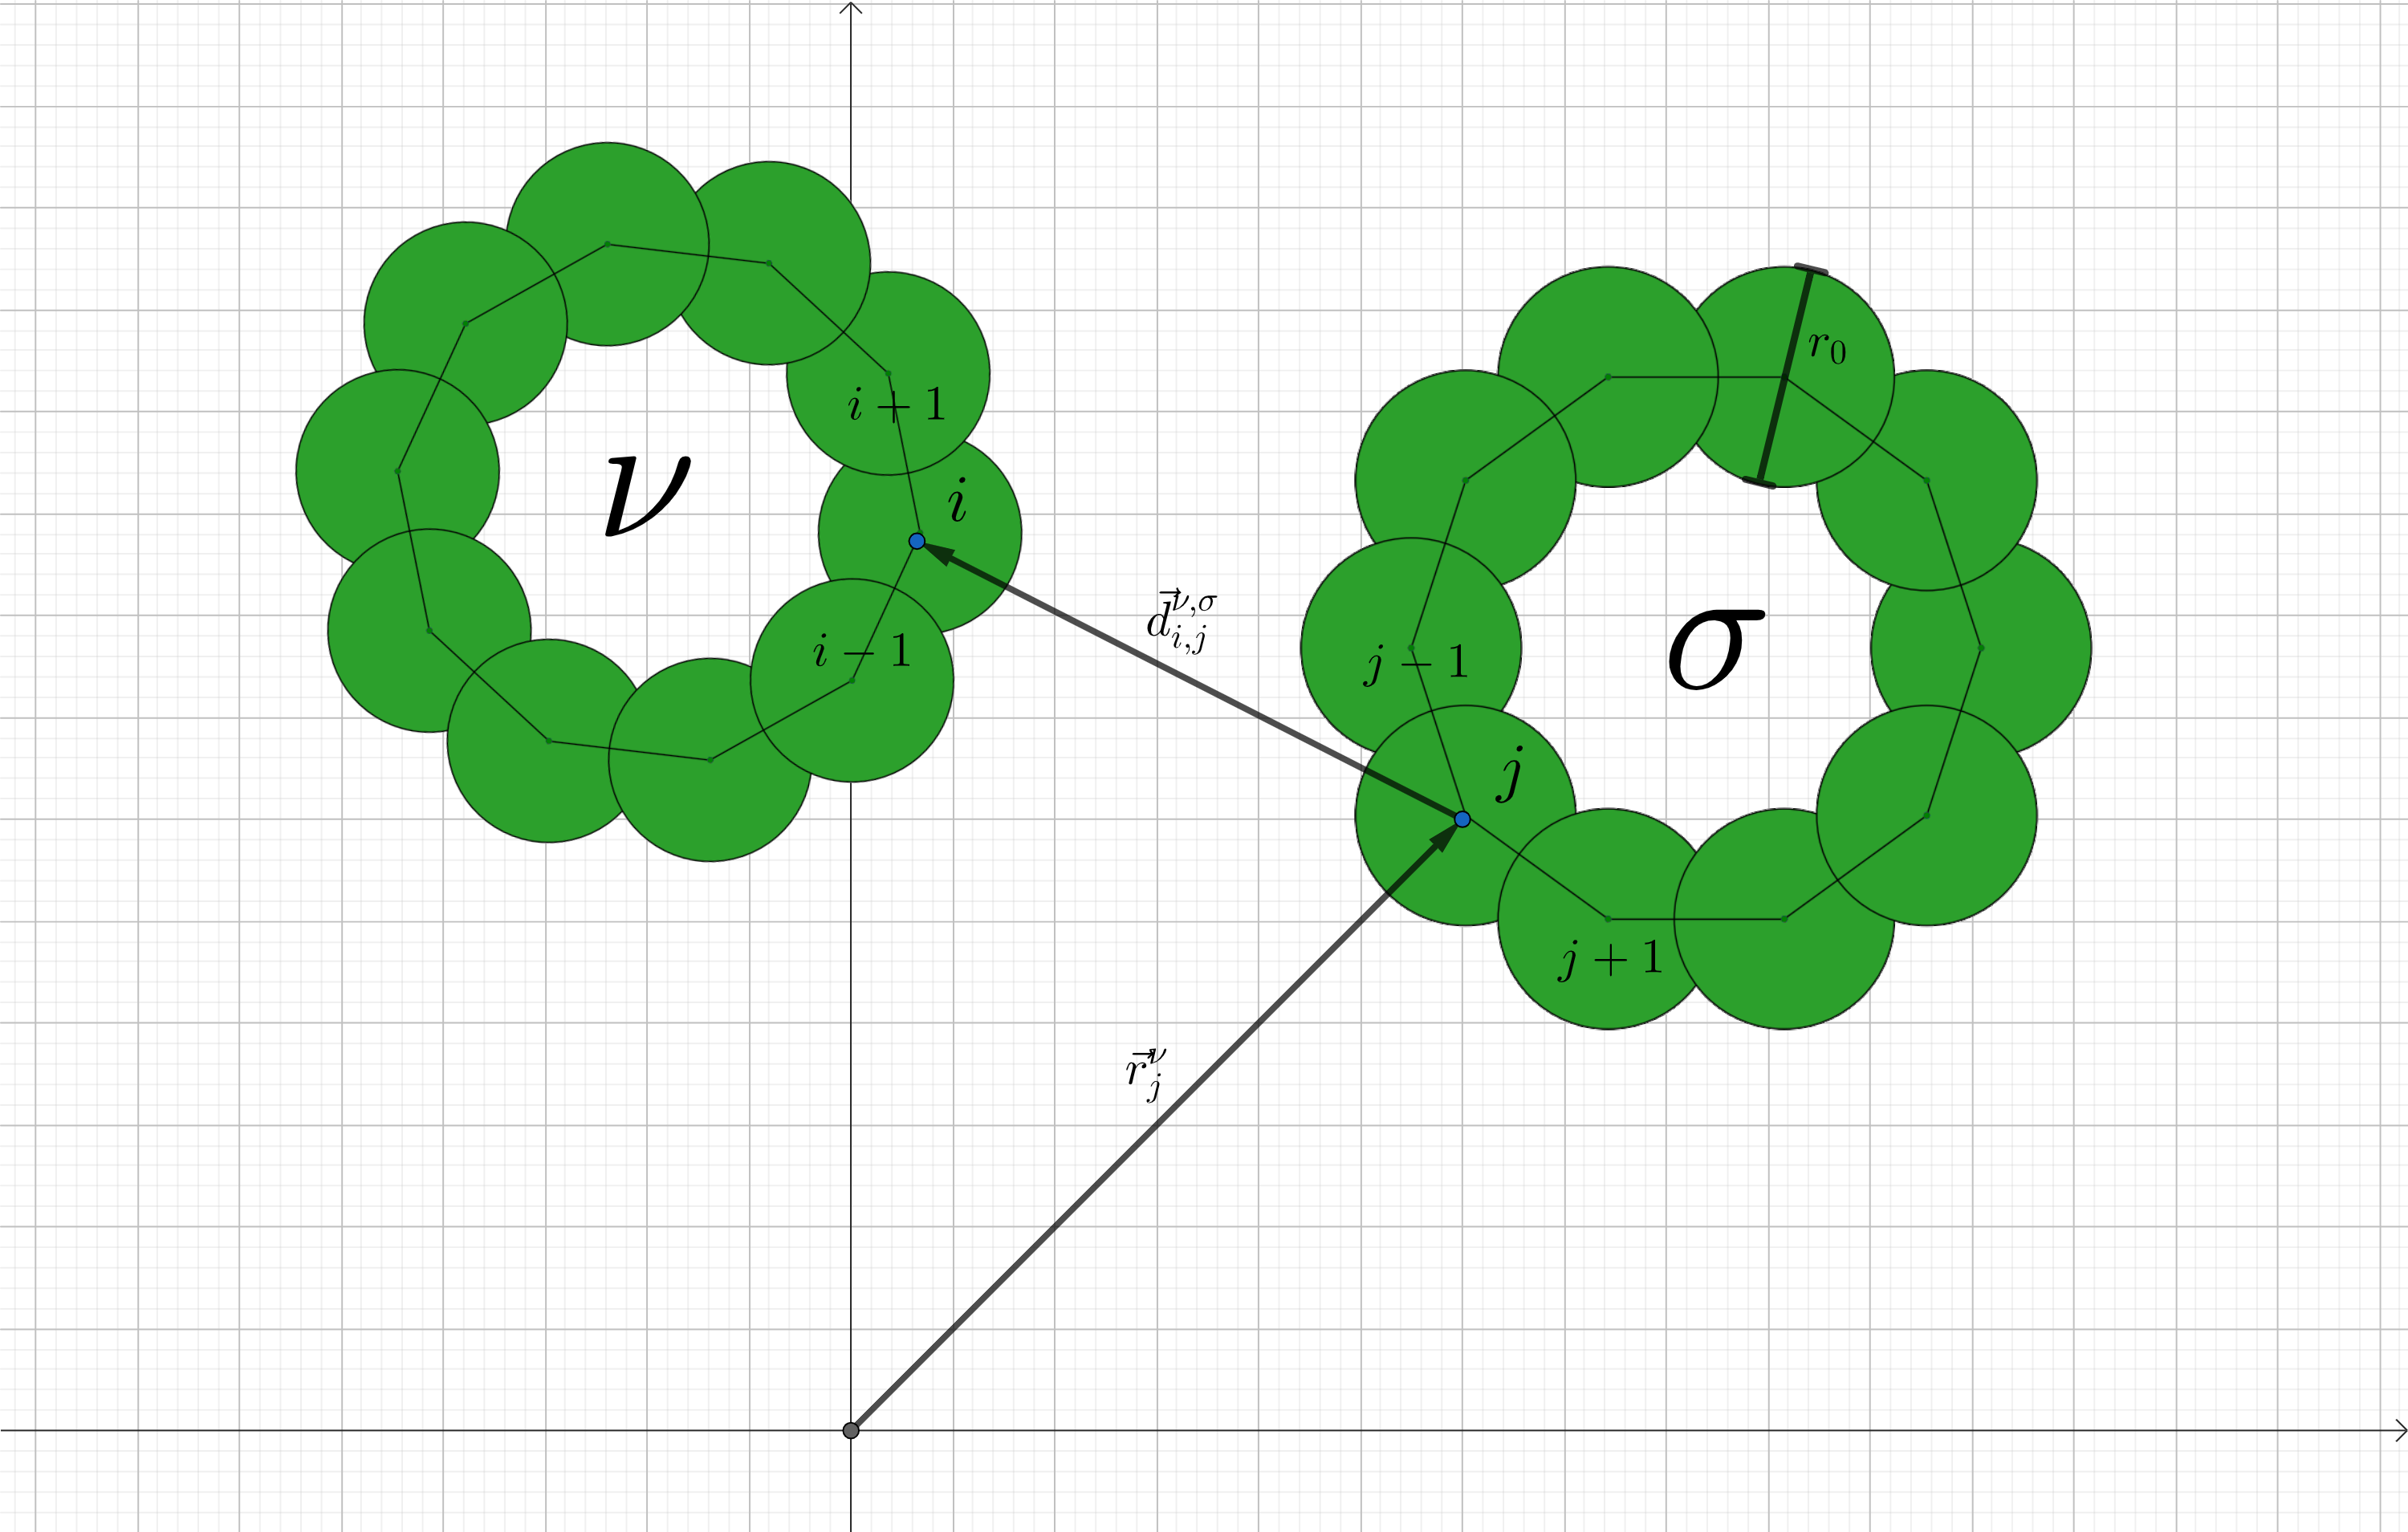
\includegraphics[width=\linewidth]{figuras/rings_diagram.png}
    \caption{Diagrama de dois anéis (anéis $\nu$ e $\sigma$) com o vetor posição da partícula $j$ do anel $\sigma$ e o vetor distância de $j$ até a partícula $i$ do anel $\nu$. O diâmetro das partículas é dado por $r_0$ (eq. [\ref{eq:particle_particle_pot}]).}
    \label{fig:rings_diagram}
\end{figure}

A energia potencial proveniente da mola que conecta as partículas ($i-1$) e $i$ no anel $\nu$ é

\begin{equation}
    {\{U_m\}}_{i}^{\nu} = \frac{k_m}{2}(\deslocsc{i}{\nu} - l_0)^2
\label{eq:spring_pot}
\end{equation}
em que $k_m$ é a constante da mola e $l_0$ seu comprimento de equilíbrio.

A próxima energia dá origem a uma força que tende a preservar a área dos anéis, para escrevê-la precisamos da área do anel $\nu$, que pode ser calculada com a seguinte expressão \footnote{O módulo da expressão da área (eq. [\ref{eq:ring_area}]) pode ser retirado contanto que a iteração das partículas seja feita no sentido anti-horário.}

\begin{equation}
    A_\nu = \frac{1}{2}\norm{\sum_{i=1}^{n}\pos{i}{\nu} \times \pos{i+1}{\nu}}\;,
\label{eq:ring_area}
\end{equation}
a energia potencial associada a força que tende a preservar a área do anel $\nu$ em torno de uma área alvo $A_0$ é dada por

\begin{equation}
    {\{U_A\}}_{\nu} = \frac{k_a}{2}(A_{\nu} - A_0)^2
\label{eq:area_pot}
\end{equation}
em que $k_a$ é um parâmetro que controla a intensidade do potencial. As molas tendem a fazer com que o anel assuma o formato de um polígono regular de lado $l_0$, que corresponde a área dada pela equação [\ref{eq:spring_area}]. 

\begin{equation}
    A_m = \frac{1}{4}n{l_0}^2\cot\bigg(\frac{\pi}{n}\bigg)
    \label{eq:spring_area}
\end{equation}
Por outro lado, o parâmetro $A_0$ define independentemente uma área alvo para o anel, conforme esses valores a membrana pode apresentar-se muito esticada (caso em que $A_0 > A_m$) ou enrugada (no caso contrário). No caso $A_0 > A_m$, a área do anel irá estabilizar em um valor $A_{eq}$ tal que $A_0 > A_{eq} > A_m$. Se $A_0 < A_m$, então $A_{eq} = A_0$.
Ou seja, a relação entre $A_0$ e $A_m$ controla a deformabilidade da membrana do anel. Para explicitar essa propriedade do anel, define-se o parâmetro $p_0$ \cite{bi_motility-driven_2016},

\begin{equation}
    p_0 := \frac{P}{\sqrt{A_0}} = \frac{n l_0}{\sqrt{A_0}}
    \label{eq:p0}
\end{equation}
em que $P = n l_0$ é o perímetro definido pelas distâncias de equilíbrio das molas que unem as partículas de cada anel. Todos os anéis com o mesmo valor de $p_0$, independente do seu tamanho, vão possuir o mesmo grau de deformabilidade em suas membranas (pois $A_m/A_0$ será uma constante para $n >> 1$).
Portanto, é conveniente partir do valor de $p_0$ e obter o valor de $A_0$ através da equação [\ref{eq:p0}].

Por fim, existe uma energia potencial associada a interação entre a partícula $i$ do anel $\nu$ com a partícula $j$ do anel $\sigma$. Esse potencial apenas depende da distância entre as partículas ($\deslocgsc{i}{j}{\nu}{\sigma}$) e tem um papel semelhante a um potencial Lennard-Jones: possui uma região de repulsão quando $\deslocgsc{i}{j}{\nu}{\sigma}$ é menor do que a distância de equilíbrio ($r_0$), e uma região de adesão quando $r_0 < \deslocgsc{i}{j}{\nu}{\sigma} < r_0 + b$, onde $b$ é o comprimento da região de adesão. $r_0$ acaba sendo o diâmetro efetivo das partículas. Tal potencial é descrito pela equação, %[\ref{eq:particle_particle_pot}]

\begin{equation}
\begin{aligned}
{\{U_p\}}_{i, i-1}^{\nu, \nu} &= {\{U_p\}}_{i, i}^{\nu, \nu} = {\{U_p\}}_{i, i+1}^{\nu, \nu} = 0, ~\forall~i, \nu \\
{\{U_p\}}_{i, j}^{\nu, \sigma} &= \begin{cases}
    \frac{k_{rep}}{2r_0}(\deslocgsc{i}{j}{\nu}{\sigma} - r_0)^2 &, 0 \leq \deslocgsc{i}{j}{\nu}{\sigma} \leq r_0 \\
    \frac{k_{atr}}{2b}(\deslocgsc{i}{j}{\nu}{\sigma} - r_0)^2 &, r_0 < \deslocgsc{i}{j}{\nu}{\sigma} < r_0 + b \text{ e } \nu \neq \sigma \\
    0 &, r_0 < \deslocgsc{i}{j}{\nu}{\sigma} < r_0 + b \text{ e } \nu = \sigma \\
    0 &, \deslocgsc{i}{j}{\nu}{\sigma} \geq r_0 + b 
\end{cases}
\end{aligned}
\label{eq:particle_particle_pot}
\end{equation}
onde $k_{rep}$ e $k_{atr}$ controlam a intensidade das forças de repulsão e adesão, respectivamente. Note que partículas vizinhas em um mesmo anel não contribuem para esse potencial, ou seja, elas apenas interagem através da mola que as conecta. Ainda, partículas no mesmo anel (que não são vizinhas) apenas repelem-se quando dentro de uma distância $r_0$, sem qualquer atração. 

A energia potencial total do sistema ($U$) pode ser escrita da seguinte forma
\begin{equation}
\begin{aligned}
    U_m &= \sum_{\nu=1}^N\sum_{i=1}^{n} {\{U_m\}}_i^\nu \\
    U_A &= \sum_{\nu=1}^N {\{U_A\}}_\nu \\
    U_p &= \sum_{\nu < \sigma}^N \sum_{i, j}^n {\{U_p\}}_{i, j}^{\nu,   \sigma}  + \sum_{\nu=1}^N\sum_{i < j}^n {\{U_p\}}_{i, j}^{\nu, \nu}\\
    U & = U_m + U_A + U_p
\end{aligned}
\label{eq:total_energy}
\end{equation}

\subsection{Forças}
\paragraph{}
Estando definidas as expressões das energias, podemos derivá-las para obter as forças.

\subsubsection{Partículas vizinhas}
\paragraph{}
A força exercida na partícula $i$ no anel $\nu$ pelas suas vizinhas imediatas é
\begin{equation}
\begin{aligned}
    \quantity{\{F_m\}}{i}{\nu} &= -\quantitysc{\nabla}{i}{\nu}U_m = -\quantitysc{\nabla}{i}{\nu}\bigg[\quantitysc{\{U_m\}}{i}{\nu} + \quantitysc{\{U_m\}}{i+1}{\nu} \bigg] = \\ 
    &= -k_m (\deslocsc{i}{\nu} -l_0)\frac{\desloc{i}{\nu}}{\deslocsc{i}{\nu}} + k_m (\deslocsc{i+1}{\nu} -l_0)\frac{\desloc{i+1}{\nu}}{\deslocsc{i+1}{\nu}}
\end{aligned}
\label{eq:force_spring}
\end{equation}

\subsubsection{Partícula-Partícula}
\paragraph{}
É conveniente definir uma função indicadora de vizinhos em um anel, que chamaremos de $CN$ (\textit{close neighbors}). Dada a partícula $i$ no anel $\nu$ e a partícula $j$ no anel $\sigma$,  $CN_{i, j}^{\nu, \sigma}$ é 1 se as partículas pertencem ao mesmo anel ($\sigma = \nu$) e são vizinhas ($|i - j| \leq 1$). Uma forma de definir $CN$ é a seguinte\footnote{A igualdade $j=i\pm 1$ é verdadeira se ambos os índices se referem a mesma partícula, por exemplo, n = 0 resulta em verdadeiro.}
% \begin{equation}
%     CN_{i, j}^{\nu, \sigma} = \begin{cases}
%         1,& \nu = \sigma \text{ e } |i - j| - \max\{0,  2(|i-j| - \lceil \frac{n}{2} \rceil) + n\bmod2 \} \leq 1 \\
%         0,& \text{caso contrário}
%     \end{cases}
% \label{eq:close_neihbors}
% \end{equation}
% outra possível forma é \footnote{A igualdade $j=i\pm 1$ é verdadeira se ambos os índices se referem a mesma partícula, por exemplo, n = -1 resulta em verdadeiro.}
\begin{equation}
CN_{i, j}^{\nu, \sigma} = \begin{cases}
        1,& (\nu = \sigma) \text{ e } (j=i \text{ ou } j = i \pm 1) \\
        0,& \text{caso contrário}
    \end{cases}
    \label{eq:close_neihbors}
\end{equation}
Repare que a própria partícula é considerada como sua vizinha. Agora considere o conjunto de índices de partículas que estão a uma distância menor ou igual a $r_0$ em relação a partícula $i$ no anel $\nu$, e que não são vizinhas de $i$ 
\[
B_{rep} := \{(j, \sigma)~|~ \deslocgsc{i}{j}{\nu}{\sigma} \leq r_0 \text{ e } CN_{i, j}^{\nu, \sigma} = 0 \}
\]
também considere o conjunto de índices de partículas em diferentes anéis, que estão a uma distância maior do que $r_0$ e menor do que $r_0 + b$ em relação a partícula $i$ no anel $\nu$
\[
B_{adh} := \{(j, \sigma)~|~ r_0 < \deslocgsc{i}{j}{\nu}{\sigma} < r_0+b \text{ e } \nu \neq \sigma\}
\]
então a força de interação partícula-partícula atuando na partícula $(i, \nu)$ pode ser escrita como

\begin{equation}
\begin{aligned}
    \quantity{\{F_p\}}{i}{\nu} = &- \quantitysc{\nabla}{i}{\nu} U_p = \\ 
    = &-\sum_{(j, \sigma) \in B_{rep}} \frac{k_{rep}}{r_0}(\deslocgsc{i}{j}{\nu}{\sigma} - r_0)\frac{\deslocg{i}{j}{\nu}{\sigma}}{\deslocgsc{i}{j}{\nu}{\sigma}} ~~-\\
    &-\sum_{(j, \sigma) \in B_{adh}} \frac{k_{adh}}{b}(\deslocgsc{i}{j}{\nu}{\sigma} - r_0)\frac{\deslocg{i}{j}{\nu}{\sigma}}{\deslocgsc{i}{j}{\nu}{\sigma}}
\end{aligned}
\label{eq:force_particle_particle}
\end{equation}

\subsubsection{Preservação da área}
\paragraph{}
A força que preserva a área do anel $\nu$ atuando na partícula $i$ é

\[    
\quantity{\{F_A\}}{i}{\nu} = - \quantitysc{\nabla}{i}{\nu}U_A = -\quantitysc{\nabla}{i}{\nu} \{U_A\}_\nu
\]
desenvolvendo o gradiente, concluímos que a força é
\begin{equation}
    \quantity{\{F_A\}}{i}{\nu} = \frac{1}{2}k_a (A_\nu - A_0) R_{\pi/2}\big( \quantity{r}{i+1}{\nu} - \quantity{r}{i-1}{\nu}\big)
\label{eq:force_area}
\end{equation}
em que $R_{\pi/2}$ é a matriz de rotação em $\pi/2$ radianos no sentido anti-horário
\[
    R_{\pi/2} = \begin{bmatrix}
        0 &-1 \\
        1 &0
    \end{bmatrix}
\]

\subsubsection{Evitando superposições}
\paragraph{}
Uma das consequências de construir membranas usando partículas ligadas por molas é a possibilidade de um anel invadir a área ocupado por outro anel. Esse problema acontece com muita facilidade em nossas simulações, pois existe uma região de alta pressão na situação que estamos explorando (a região logo antes do obstáculo do canal). Isso pode ser evitado aumentando as constante que mantém o anel unido e repelem partículas de diferentes anéis, mas isso também requer diminuir o passo temporal no esquema de integração. Também é possível diminuir $v_0$ para reduzir as invasões, mas isso reduz a escala de tempo da simulação. Portanto, como alternativa de remediar esse problema, sem drasticamente sacrificar o tempo de execução, foi desenvolvido uma força cujo papel é desfazer invasões em andamento. Primeiramente, vamos definir o que é uma invasão:
\begin{definition}[Invasões]
\label{def:invasion}
Dizemos que a partícula $i$ do anel $\nu$, cuja posição é posição $\quantity{r}{i}{\nu}$, está invadindo o anel $\sigma$ se $\quantity{r}{i}{\nu}$ está contida no polígono formado pelas posições das partículas do anel $\sigma$. Nesse caso $\nu$ é o anel invasor e $\sigma$ é o anel invadido.
\end{definition}
A checagem de invasões é feita através de um algoritmo de checagem de pontos dentro de polígonos utilizando a regra da paridade \cite{hormann_point_2001}. 
% A verificação de que o anel $\nu$ está invadindo $\sigma$ necessita $n^2$ checagens de intersecções entre retas. Para melhorar o seu desempenho, os anéis são divididos em caixas (da mesma forma que as partículas são divididas em caixas no cálculo da força partícula-partícula) e apenas é verificado invasões entre anéis que estão na mesma caixa ou em caixas vizinhas. 

Assim que uma invasão é detectada, digamos que $(i, \nu)$ invadiu $\sigma$, é aplicado uma força de módulo constante ($F_{inv}$) na partícula invasora, cuja direção é a mesma da força de preservação da área atuando em $i$ (eq. [\ref{eq:force_area}]). Para garantir que a força aponta para fora do anel invadido, apenas basta supor que $A_\nu < A_0$ na equação [\ref{eq:force_area}]. Para diminuir a interferência  causada por essa força, as partículas invasoras são monitoradas em todos os passos temporais até saírem de dentro do anel invadido, assim que saírem, a força anti-invasão pode desaparecer ou continuar por mais alguns passos temporais. 

\subsection{Equações de movimento}
\paragraph{}
Cada partícula é governada por equações de movimento super-amortecidas com atividade e mecanismo de auto-alinhamento. Atividade significa que a partícula tem a capacidade de se auto-propelir, a velocidade de autopropulsão tem módulo constante dado pelo parâmetro $v_0$ e orientação dada pelo vetor unitário $\hat n_\nu$, que também é chamado de polarização. No presente modelo, todas as partículas do mesmo anel possuem a mesma polarização, ou seja, existe uma única polarização associada ao anel (por isso do sub-índice $\nu$ em $\hat n_\nu$), logo o anel como um todo tem uma direção e sentido na qual ele se auto-propele. 

O mecanismo de auto-alinhamento surge do seguinte processo: a polarização do anel tende a relaxar em direção a velocidade do anel ($\vec v_\nu$), que é dada pela média das velocidade de suas partículas 
\begin{equation}
\vec v_{\nu} := \frac{1}{n} \sum_{i=1}^n \frac{d}{dt}\pos{i}{\nu}
\label{eq:vel_cm}
\end{equation}
O tempo característico de relaxamento é dado pelo parâmetro $\tau$, se $\tau$ é muito pequeno, os anéis alinham suas velocidades quando entram em contanto.
Além da velocidade da partícula ser proporcional a sua atividade, ela também é proporcional às forças externas, pois estamos assumindo que as células estão em um meio muito viscoso, com efeitos inercias desprezíveis.

Define-se $\theta_\nu$ como o ângulo da polarização ($\hat n_\nu = (cos(\theta_\nu), sen(\theta_\nu))$) e atribui-se  ruído branco gaussiano em $\theta_\nu$ para simular o comportamento assintótico de caminhada aleatória para os anéis. O parâmetro $D_r$ controla a intensidade do ruído.

As seguintes equações de movimento encapsulam todos os mecanismos recém discutidos:
\begin{equation}
\begin{aligned}
\frac{d}{dt}\pos{i}{\nu} &= v_o \hat n_\nu(t) - \mu \nabla_i^\nu U \\
\frac{d}{dt}\theta_{\nu} &= \frac{1}{\tau}\arcsin\bigg(\hat n_\nu(t) \times \frac{\vec v_{\nu}}{v_{\nu}} \cdot \hat e_z \bigg) + \sqrt{2 D_R}\xi_\nu(t)
\end{aligned}
\label{eq:eq_motion}
\end{equation}
Para fins de organização, segue uma breve descrição de todos os componentes das equações de movimento:
\begin{itemize}
    \item $\frac{d}{dt}\pos{i}{\nu}$: Velocidade da partícula $i$ no anel $\nu$.
    \item $\hat n_\nu$: Polarização do anel $\nu$.
    \item $\theta_\nu$: Ângulo da polarização.
    \item -$\nabla_i^\nu$U: Força exercida sobre a partícula $i$ no anel $\nu$.
    \item $v_o$: Magnitude da velocidade autopropulsora. 
    \item $\mu$: Mobilidade. 
    \item $\tau$: Tempo de relaxamento entre $\hat n_\nu$ e $\vec v_\nu$. 
    \item $D_R$: Coeficiente de difusão rotacional.
    \item $\xi_\nu(t)$: Ruído branco gaussiano satisfazendo média zero e correlacionado por deltas
    $$\langle \xi_\nu(t_1) \xi_\sigma(t_2) \rangle = \delta_{\nu \sigma}\delta(t_1 - t_2)$$
\end{itemize}


\section{Metodologia}
\paragraph{}
Para explorar o modelo dos anéis ativos, simulamos um fluxo de anéis, com 10 partículas cada, em um canal retangular com obstáculo circular centrada em seu centro (geometria de Stokes), integrando as equações de movimento (eq. [\ref{eq:eq_motion}]) através do método de Euler.  Daqui em diante, $\Delta t$ denotará o passo temporal do esquema de integração.

\subsection{Fontes e sumidouros do fluxo de anéis}
\paragraph{}
Nossas simulações começam com o canal completamente vazio, então, para estabelecer o fluxo, anéis são criados em uma região retangular no inicio do canal sempre que existe espaço disponível, e, enquanto permanecem nessa região, são empurrados em direção ao obstáculo através de uma força horizontal constante, cujo módulo é um parâmetro da simulação ($F_i$). Quando anéis penetram uma região no final do canal, eles são removidos do sistema.

\subsection{Dimensões do canal}
\paragraph{}
As dimensões geométricas do canal são dadas em função do diâmetro de equilíbrio dos anéis ($d_{eq}$), que é o comprimento assumido pelo anel quando não está sob a influência de forças externas. $d_{eq}$ pode depender do comprimento de equilíbrio das molas que conectam as partículas em um anel ($l_0$) e da área de equilíbrio do potencial responsável por preservar a área do anel ($A_0$). O diâmetro de equilíbrio é calculado assumindo que o anel possui a forma de um círculo, ou seja,

\begin{equation}
    d_{eq} = 2\sqrt{\frac{A_{eq}}{\pi}}
    \label{eq:ring_d_eq}
\end{equation}
em que $A_{eq}$ é a área do anel quando não está sob a influência de forças externas. As dimensões utilizadas para o canal em todas as simulações estão na tabela \ref{tab:channel_dims}. A figura \ref{fig:channel_view} contém uma ilustração do canal destacando todas suas regiões e informando suas dimensões.

\begin{table}[h]
    \centering
    \begin{tabular}{|| l || c ||} 
     \hline
     Comprimento & 200 $d_{eq}$ \\
     \hline
     Altura & 50 $d_{eq}$ \\
     \hline
     Diâmetro do obstáculo & 15 $d_{eq}$ \\
     \hline
    \end{tabular}
    \caption{Tamanho do canal e de seu obstáculo utilizados nas simulações, dados em função do diâmetro de equilíbrio dos anéis $d_{eq}$.}
    \label{tab:channel_dims}
\end{table}

\begin{figure}[h]
    \centering
    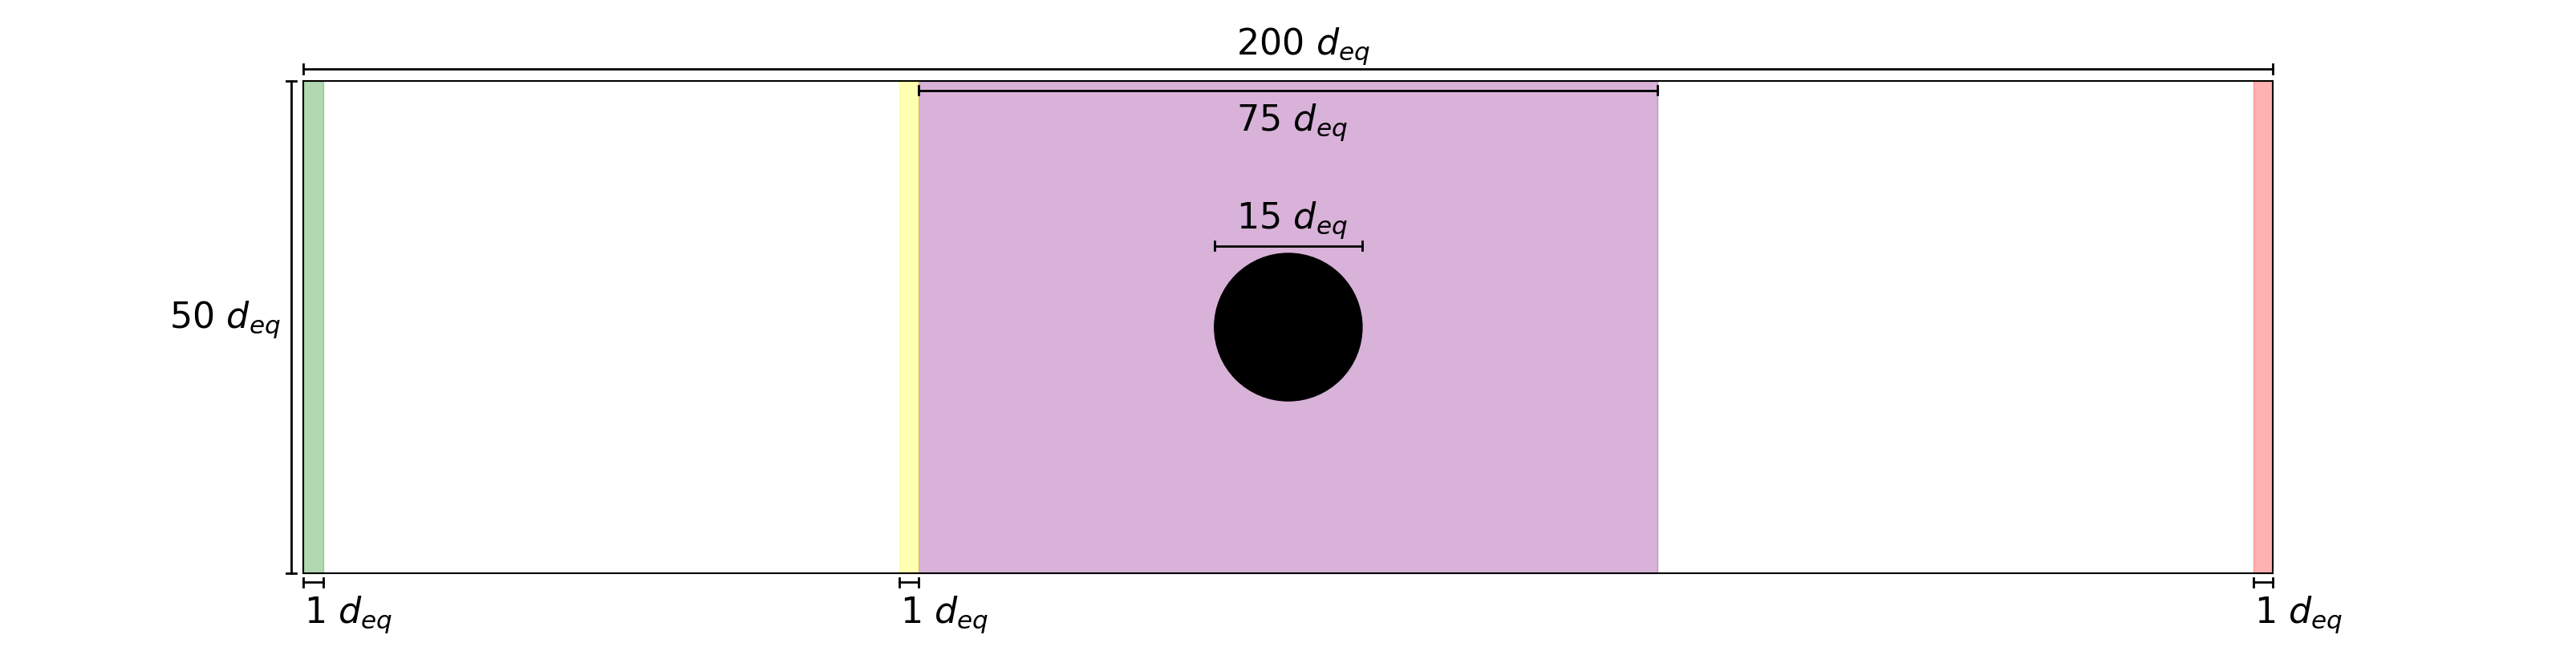
\includegraphics[width=\linewidth]{figuras/channel_dims.png} 
    \caption{Ilustração do canal com suas dimensões dadas em relação ao diâmetro de equilíbrio dos anéis ($d_{eq}$). A região verde é onde os anéis são criados (região de criação), a vermelha onde os anéis são removidos (região de remoção), a amarela é a região das medidas de entrada e a roxa a região das medidas de saída. O círculo preto é o obstáculo do canal.}
    \label{fig:channel_view}
\end{figure}

\subsection{Obstáculo e bordas do Canal}
\paragraph{}
O obstáculo circular no canal possui um centro ($\vec p_{obs}$) e um raio ($r_{obs}$). Quando uma partícula adentra sua área, uma força é aplicada na mesma, de acordo com a equação [\ref{eq:obs_force}]

\begin{equation}
  \vec F_{obs, i, \nu} = \begin{cases}
      k_{obs} \big(r_{obs} - \norm{\pos{i}{\nu} - \vec p_{obs}} \big) \frac{\big( \pos{i}{\nu} - \vec p_{obs} \big)}{\norm{\pos{i}{\nu} - \vec p_{obs}}} &, ~ \norm{\pos{i}{\nu} - \vec p_{obs}} < r_{obs} \\
       0 &, ~\textit{Caso contrário}
  \end{cases}  
\label{eq:obs_force}
\end{equation}
em que $k_{obs}$ é um parâmetro que controla a intensidade dessa força.

As bordas do canal são tratadas da seguinte forma: Se uma partícula sai do canal por alguma borda, a componente da velocidade perpendicular a essa borda é zerada, caso ela aponte para fora da borda. 


\subsection{Preparação da condição inicial}
\paragraph{}
Para reduzir o tempo de execução, uma condição inicial que preenche todo o canal foi preparada, e todos as demais simulações começaram a partir dela. Ele é de grande ajuda principalmente nos casos em que o alinhamento é baixo ($\tau$ muito grande). Os parâmetros utilizados para gerar essa configuração estão na tabela \ref{tab:init_cond_pars} e a simulação rodou até o tempo final $6000$. 

É importante ressaltar que as simulações que começaram a partir dessa configuração inicial modificaram os parâmetros da tabela \ref{tab:init_cond_pars} de acordo com a situação a ser explorada.

\begin{table}[h]
    \centering
    \begin{subtable}[t]{0.48\textwidth}
        \centering
        \begin{tabular}[t]{||c|c||}
        \hline
        \multicolumn{2}{|c|}{\textbf{Forças}} \\
        \hline 
        Parâmetro & Valor \\
        \hline \hline
        $k_m$ & 28 \\ \hline
        $l_0$ & 0.7 \\ \hline
        $k_a$ & 4 \\ \hline
        $p_0$ & 4 \\ \hline
        $r_0$ & 1 \\ \hline
        $b$ & 0.05 \\ \hline
        $k_{rep}$ & 20 \\ \hline
        $k_{atr}$ & 1 \\ \hline
        $F_i$ & 0.5 \\ \hline
        $k_{obs}$ & 25 \\ \hline
        $F_{inv}$ & 11 \\ \hline
        \end{tabular}
        % \caption{Caption 1}
        \label{tab:init_cond_pars_force}
    \end{subtable}
    \hspace{\fill}
    \begin{subtable}[t]{0.48\textwidth}
        \begin{subtable}[t]{\textwidth}
            \centering
            \begin{tabular}[t]{||c|c||}
                 \hline
                 \multicolumn{2}{|c|}{\textbf{Equações de movimento}} \\
                 \hline
                 Parâmetro & Valor \\
                 \hline \hline
                 $\tau$ & 1 \\ \hline
                $\mu$ & 1 \\ \hline
                $v_0$ & 0.5 \\ \hline
                $D_r$ & 1 \\ \hline
                $\Delta t$ & 0.01 \\ \hline
            \end{tabular}
            % \caption{Caption 2}
            \label{tab:init_cond_pars_eq_motion}
        \end{subtable}
    \end{subtable}
    \caption{Parâmetros utilizados para construir a condição inicial utilizada como ponto de partida de todas as outras simulações.}
    \label{tab:init_cond_pars}
\end{table}

% \begin{table}[h]
%     \centering
%     \begin{tabular}{||c|c||}
%         \hline
%         Parâmetro & Valor \\
%         \hline \hline
%         $k_m$ & 28 \\
%         \hline
%         $l_0$ & 0.7 \\
%         \hline
%         $k_a$ & 4 \\
%         \hline
%         $p_0$ & 4 \\
%         \hline
%         $k_{inv}$ & 11 \\
%         \hline
%         $r_0$ & 1 \\
%         \hline
%         $b$ & 0.05 \\
%         \hline
%         $k_{rep}$ & 20 \\
%         \hline
%         $k_{atr}$ & 1 \\
%         \hline
%         $F_i$ & 0.5 \\
%         \hline
%         $\tau$ & 1 \\
%         \hline
%         $\mu$ & 1 \\
%         \hline
%         $v_0$ & 0.5 \\
%         \hline
%         $D_r$ & 1 \\
%         \hline
%     \end{tabular}
%     \caption{Parâmetros utilizados para gerar a condição inicial.}
%     \label{tab:init_cond_pars}
% \end{table}

\subsection{Método de exploração}
\paragraph{}
Para explorar o comportamento dos anéis ativos, escolhemos um conjunto de quantidades de interesse e associamos a cada uma delas um parâmetro do modelo que esperamos controlá-la. As seguintes quantidades e parâmetros foram selecionados: 
\begin{itemize}
    \item Densidade: Intensidade da força que empurra os anéis no início do canal ($F_i$).
    \item Adesão/Tensão entre anéis: Constante do potencial partícula-partícula na região de adesão ($k_{atr}$).
    \item Alinhamento da velocidade dos anéis: Tempo de relaxação ($\tau$).
\end{itemize}
Simulamos as configurações extremas dos parâmetros selecionados, mantendo todos os outros fixos. Uma configuração é dita extrema quando os valores dos parâmetros estão perto de seu limite superior ou inferior. O parâmetro pode ser limitado por questões físicas (por exemplo, $\tau$ deve ser um valor positivo) ou por questões numéricas (por exemplo, valores muito altos para $F_i$ resultam em erros numéricos inaceitáveis). Dessa forma, existem 8 configurações para serem simuladas, que denotaremos da seguinte forma:
\begin{center}
A[0 ou 1]-D[0 ou 1]-T[0 ou 1] 
\end{center}
em que "A" significa alinhamento, "D" densidade, "T" adesão/tensão e 0 condiz com o parâmetro em um valor que minimiza a respectiva quantidade e 1 com um valor que maximiza, por exemplo, A1-D0-T1 representa uma configuração com alinhamento alto (correspondendo a um valor baixo para $\tau$), densidade baixa (correspondendo a um valor baixo para $F_i$) e tensão/força alta (correspondendo a um valor alto para $k_{atr}$). 

\subsubsection{Parâmetros fixos}
\paragraph{}
Os parâmetros fixos utilizados em todas as simulações estão na tabela \ref{tab:fix_pars}.
\begin{table}[h]
    \centering
    \begin{tabular}{||c|c|l||}
        \hline
        Parâmetro & Valor & Descrição \\
        \hline \hline
        $k_m$ & 28 & Constante das molas \\
        \hline
        $l_0$ & 0.8 & Comprimento de equilíbrio das molas \\
        \hline
        $k_a$ & 13 & Constante da força de preservação de área \\
        \hline
        $p_0$ & 3.6051 & Flexibilidade da membrana do anel \\
        \hline
        $r_0$ & 1 & Diâmetro das partículas \\
        \hline
        $b$ & 0.18 & Tamanho da região da adesão \\
        \hline
        $k_{rep}$ & 28 & Constante da força de repulsão entre partículas \\
        \hline
        $\mu$ & 1 & Mobilidade \\
        \hline
        $v_0$ & 0.5 & Atividade \\
        \hline
        $D_r$ & 0.25 & Ruído rotacional \\
        \hline
        $k_{obs}$ & 30 & Força do obstáculo \\
        \hline
        $F_{inv}$ & 28 & Força anti-invasão \\
        \hline
        $\Delta t$ & 0.01 & Passo temporal na integração \\
        \hline
    \end{tabular}
    \caption{Parâmetros fixos utilizados em todas as simulações.}
    \label{tab:fix_pars}
\end{table}
Conforme já comentado, um problema muito comum com o presente modelo é um anel invadir outro anel, esse problema pode ser evitado aumentando $k_m$, dificultando o afastamento entre partículas vizinhas no mesmo anel, porém isso acaba por aumentar a força com que uma partículas é empurrada contra outro anel, portanto também é necessário aumentar $k_{rep}$ para que a partícula invasora não atravesse por cima das partículas do anel sendo invadido. Setamos $k_m$ e $k_{rep}$ para o maior possível sem causar problemas numéricos aparentes.

É desejável que a superfície de contato entre anéis tenha protuberâncias, no melhor dos casos teríamos $l_0 = r_0$, no entanto essa configuração é muito propícia para invasões entre anéis, pois é fácil abrir espaço entre as partículas vizinhas, então optamos por escolher um valor de $l_0$ um pouco menor do que $r_0$.

A flexibilidade da membrana do anel depende da razão entre $A_0$ e $A_m$. Optamos por escolher o caso limite entre membrana rígida ($A_0 > A_m$) e flexível ($A_0 < A_m$), ou seja, quando $A_m = A_0$, que corresponde a $p_0 = 3.6051$.

Setamos o valor de $k_a$ até o desvio da área do anel em relação ao seu valor de equilíbrio (que no nosso caso é $A_{eq}=A_0$) ser $20\%$ no pior dos casos.

\subsubsection{Limites extremos dos parâmetros variáveis}
\paragraph{}
O alinhamento, controlado por $\tau$, deve ser ao menos um pouco maior do que $\Delta t = 0.01$, então escolhemos como limite inferior $100 \cdot \Delta t = 1$. O limite superior foi definido em 50.

A densidade, controlada pela força que empurra os anéis no início do canal ($F_i$), deve ser maior do que 0 para induzir um fluxo no canal, mas não pode ser muito grande, pois isso gera pressões muito altas logo antes do obstáculo, causando erros numéricos. Os valores limites escolhidos foram 0.5 e 4.

Por fim, a adesão/tensão, controlada por $k_{atr}$, deve ser maior do que 0, pois sempre queremos que exista um pouco de adesão, mas não pode ser muito alta, pois isso gera artefatos na forma de vibração entre partículas. Os valores limites escolhidos foram 0.5 e 3. 
A tabela \ref{tab:extreme_pars_values} contém os valores selecionados para os parâmetros variáveis.

\begin{table}[h]
    \centering
    \begin{tabular}{||c|c|c|l||}
        \hline
         Parâmetro& Valor Mínimo & Valor Máximo & Quantidade associada \\ \hline \hline
         $\tau$ & 1 & 50 & Alinhamento (eq. [\ref{eq:input_alignment}]) \\ \hline
         $F_i$ & 0.5 & 4 & Densidade (eq. [\ref{eq:rel_den}])\\ \hline
         $k_{atr}$ & 0.5 & 3 & Adesão entre anéis \\ \hline
    \end{tabular}
    \caption{Valores máximos e mínimos dos parâmetros variáveis.}
    \label{tab:extreme_pars_values}
\end{table}

\subsection{Medidas}
\paragraph{}
Durante a simulação, são feitas dois tipos de medidas: medidas de entrada e medidas de saída.

\subsubsection{Medidas de saída}
\paragraph{}
São os resultados obtidos da simulação que caracterizam o fluxo de anéis. Após um período transite, quando o fluxo foi estabilizado no canal, as medidas de saída são realizadas em uma região centrada no obstáculo (região roxa na figura \ref{fig:channel_view}), dividindo a mesma em caixas retangulares. As dimensões dessa região está informada na figura \ref{fig:channel_view}.  Em cada caixa, a quantidade em questão é calculada, assim gerando um mapa espacial. O seguinte conjunto de quantidades formam as medidas de saída:

\begin{itemize}
    \item Densidade relativa ($\delta \rho$): Densidade relativa ao seu valor de equilíbrio 
    \begin{equation}
    \delta \rho = \frac{\rho}{\rho_{eq}} - 1
    \label{eq:rel_den}
    \end{equation}
    em que $\rho$ é o número de anéis por unidade de área e $\rho_{eq}$ seu valor de equilíbrio. $\rho_{eq}$ é a densidade obtida quando o espaço é preenchido por anéis em seu estado de equilíbrio quando isolados, ou seja, $\rho_{eq} = 1 / A_{eq}$. No nosso caso, $\delta \rho$ é calculado em cada caixa da região definida para realizar as medidas, e $\rho$ é o número de anéis dentro da caixa dividido pela área da caixa.
    
    \item Velocidade: Média das velocidades dos anéis que estão dentro de cada caixa.
\end{itemize}

Realizamos média temporal em todas as quantidades para melhorar a estatística dos dados.

\subsubsection{Medidas de entrada}
\paragraph{}
Para tornar possível a comparação do presente modelo com outros modelos de células móveis em fluxo de geometria de Stokes, realizamos as mesmas medidas feitas em \cite{beatrici_comparing_2023}, chamadas de medidas de entrada. Estas medidas são realizadas em uma região entre o inicio e obstáculo do canal (região amarela na figura \ref{fig:channel_view}), pois é desejável que efeitos relacionados a criação dos anéis e do obstáculo não sejam significantes. Seu propósito é monitorar o estado da simulação na entrada da região das medidas de saída e prover uma forma de verificar se diferentes modelos estão, aproximadamente, simulando a mesma situação.
As seguintes quantidades compõem o conjunto das medidas de entrada:

\begin{itemize}
    \item Alinhamento ($\phi$) \cite{vicsek_novel_1995}: Mede o quão alinhado as velocidades dos anéis estão. Seja $N$ o número de anéis dentro da região de interesse e $\vec v_{i}$ a velocidade do i-ésimo anel, então o alinhamento ($\phi$) é
    \begin{equation}
    \phi = \frac{1}{N} \norm{\sum_{i=1}^N \frac{\vec v_{i}}{v_{i}}}
    \label{eq:input_alignment}
    \end{equation}
    $\phi \approx 0$ representa fluxo desalinhado e $\phi \approx 1$ fluxo coletivo alinhado. No nosso caso, $N$ é a quantidade de anéis que estão dentro da região definida para as medidas de entrada.

    \item Densidade relativa ($\delta \rho$): A mesma densidade definida nas medidas de saída (eq. [\ref{eq:rel_den}]).

    \item Comportamento sólido-líquido ($\Delta$) \cite{gregoire_moving_2003}: Suponha que no tempo $t$ existam $N$ anéis dentro da região das medidas de entrada, e que o i-ésimo anel possua $n_i$ vizinhos. Anéis são vizinhos se eles são vizinhos no diagrama de Voronoi \cite{voronoi} construído pelos seus centros geométricos. Seja $B_i$ o conjunto de índices dos vizinhos do i-ésimo anel no tempo $t$ e $r_{ij}(t)$ a distância entre os anéis i e j no tempo $t$, então, a contribuição para $\Delta$ do i-ésimo anel é dada pela seguinte equação
    \begin{equation}
    \Delta_i = 1 - \frac{1}{n_i}\sum_{j \in B_i}\bigg(1 - \frac{r_{ij}^2(t)}{r_{ij}^2(t + T)} \bigg)
    \label{eq:delta_i}
    \end{equation}
    em que $T$ é um determinado intervalo de tempo, definido de tal forma que o centro de massa de todos os $N$ anéis tenham andado um raio do obstáculo. O $\Delta$ é dado pela média dos $\Delta_i$
    \begin{equation}
        \Delta = \frac{1}{N}\sum_{i=1}^N\Delta_i
        \label{eq:delta}
    \end{equation}
    $\Delta \approx 0$ informa que o comportamento do tecido de anéis é líquido e $\Delta \approx 1$ informa que é sólido. 
\end{itemize}
Todas as medidas de entrada são adimensionais, assim facilitando a comparação. Se diferentes modelos, em uma dada simulação, possuem aproximadamente os mesmos valores para essas medidas, eles devem estar aproximadamente simulando a mesma situação. Assim como foi feito nas medidas de saída, os dados apenas são coletados após o fluxo ser estabilizado e médias temporais são feitas para melhorar a estatística dos resultados.

% \section{Objetivos}
% \begin{itemize}
%     \item Caracterizar o fluxo de células em geometria de Stokes utilizando o modelo computacional de anéis ativos apresentado em \cite{teixeira_single_2021}, \cite{teixeira_segregation_2024}.
%     \item Comparar o modelo de anéis ativos com os outros modelos de células móveis explorados em \cite{beatrici_comparing_2023}, especialmente com o modelo de multi-partículas.
%     \item Utilizar o perfil de velocidades para comparar os nossos resultados numéricos com resultados analíticos e experimentais.
%     \item Prover uma implementação de código aberto do presente modelo, que seja de fácil instalação e esteja bem documentada.
% \end{itemize}

\section{Resultados preliminares}
\paragraph{}
Como resultados preliminares, temos as medidas de entrada e saída para os 4 casos em que o alinhamento é alto, ou seja, para os casos \case{1}{0}{0}, \case{1}{1}{0}, \case{1}{0}{1} e \case{1}{1}{1}.

Para ter noção de como o tecido de anéis estava se comportando em cada caso, a figura 
\ref{fig:vel_color_high_align} mostra um retrato da simulação centrado no obstáculo do canal, após o fluxo ter sido estabilizado. Cada partícula do anel é representada como um ponto na imagem, cuja cor é dada pelo ângulo que a velocidade do anel faz com um eixo horizontal.

\begin{figure}[h]
    \centering
    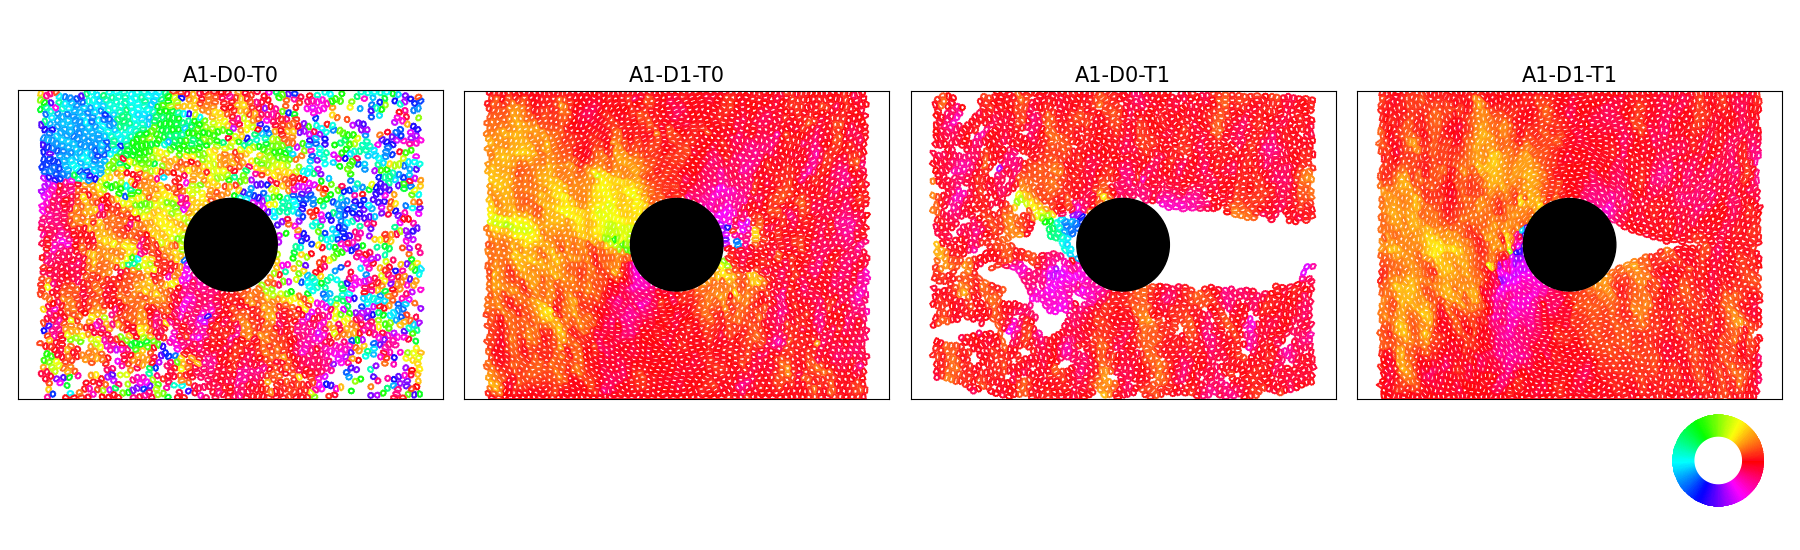
\includegraphics[width=\linewidth]{figuras/vel_color/vel_color_high_align.png}
    \caption{Visualização da simulação em um corte do canal centrado no obstáculo. Os anéis estão coloridos de acordo com o ângulo que sua velocidade faz com o eixo horizontal. O mapeamento entre ângulos e cor está indicado na roda de cor no canto direito inferior da imagem. Por exemplo, células com a cor vermelha estão se movendo para a direita.}
    \label{fig:vel_color_high_align}
\end{figure}

\FloatBarrier

\subsection{Medidas de entrada}
\paragraph{}
Comparamos nossas medidas de entrada com 3 modelos de partículas móveis, explorados no artigo original que usamos como base \cite{beatrici_comparing_2023} (figura \ref{fig:input_measurements_high_align}). Olhando para a comparação entre o modelo dos anéis (barra vermelha) e multi-partículas (barra verde), podemos notar que os anéis, em geral, alinham de forma mais eficiente e apresentam um comportamento mais sólido. A densidade relativa é aproximadamente igual, com a única exceção sendo o caso \case{1}{0}{0}, em que a densidade dos anéis é menor. 

\begin{figure}[h]
    \centering
    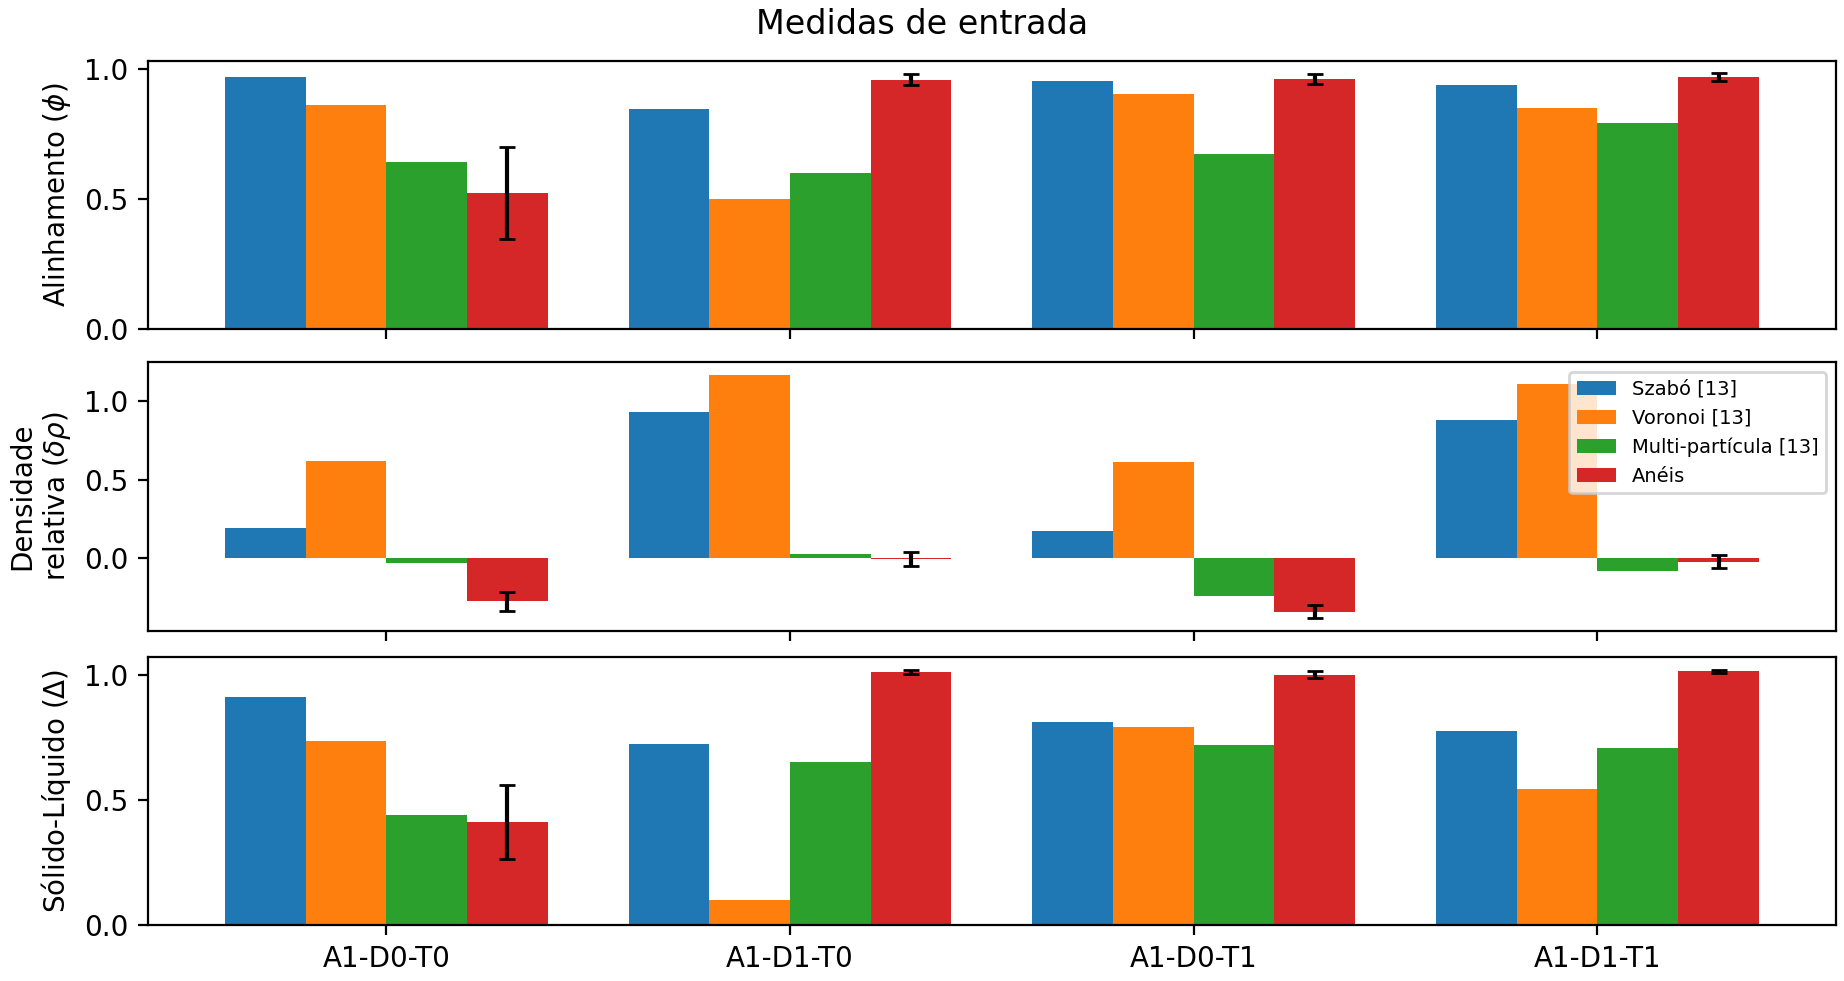
\includegraphics[width=\linewidth]{figuras/input_measurements/medidas_entrada_high_align_2.png}
    \caption{Medidas de entrada para os 4 casos em que o alinhamento é alto.}
    \label{fig:input_measurements_high_align}
\end{figure}

\subsection{Medidas de saída}
As figuras \ref{fig:output_vel_high_align} e \ref{fig:output_rel_den_high_align} contém, respectivamente, o campo de velocidades e de densidades relativas. O caso \case{1}{0}{0}, que representa uma configuração com alto alinhamento e baixos valores para os demais parâmetros, destaca-se por apresentar o menor grau de ordenamento nas velocidades. Esse comportamento é evidenciado pelas ondulações observadas no campo de velocidades.
% É notável que o caso \case{1}{0}{0}, que corresponde a uma configuração com alinhamento alto e o restante baixo, é aquele que apresenta menor ordenamento nas velocidades, como é evidenciado pelas ondulações no campo de velocidades. 
Comparando as densidades relativas nos casos \case{1}{1}{0} e \case{1}{1}{1}, observa-se que, no primeiro, o canal é completamente preenchido, enquanto, no segundo, ocorre a formação de um pequeno vazio logo após o obstáculo. Já o caso \case{1}{0}{1} apresenta um comportamento significativamente diferente dos demais: o obstáculo "racha" o tecido de anéis, resultando na formação de duas faixas distintas.

\begin{figure}[h]
    \centering
    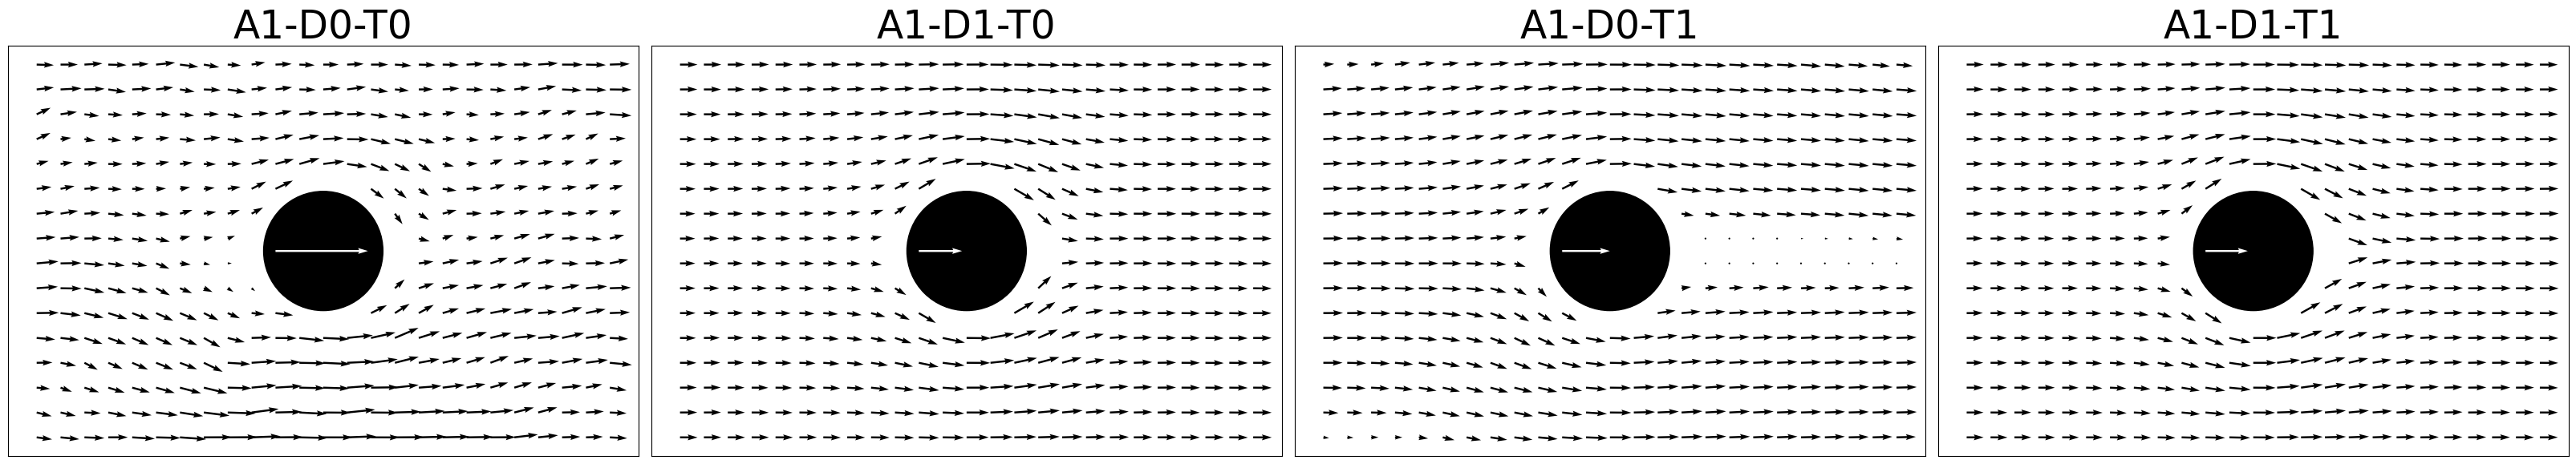
\includegraphics[width=\linewidth]{figuras/output_measurements/vel_high_align.png}
    \caption{Campo de velocidades nos casos de alinhamento alto. A seta branca dentro do obstáculo indica um vetor velocidade unitário, ou seja, a escala está diferente entre os diferentes quadros.}
    \label{fig:output_vel_high_align}
\end{figure}

\begin{figure}[h]
    \centering
    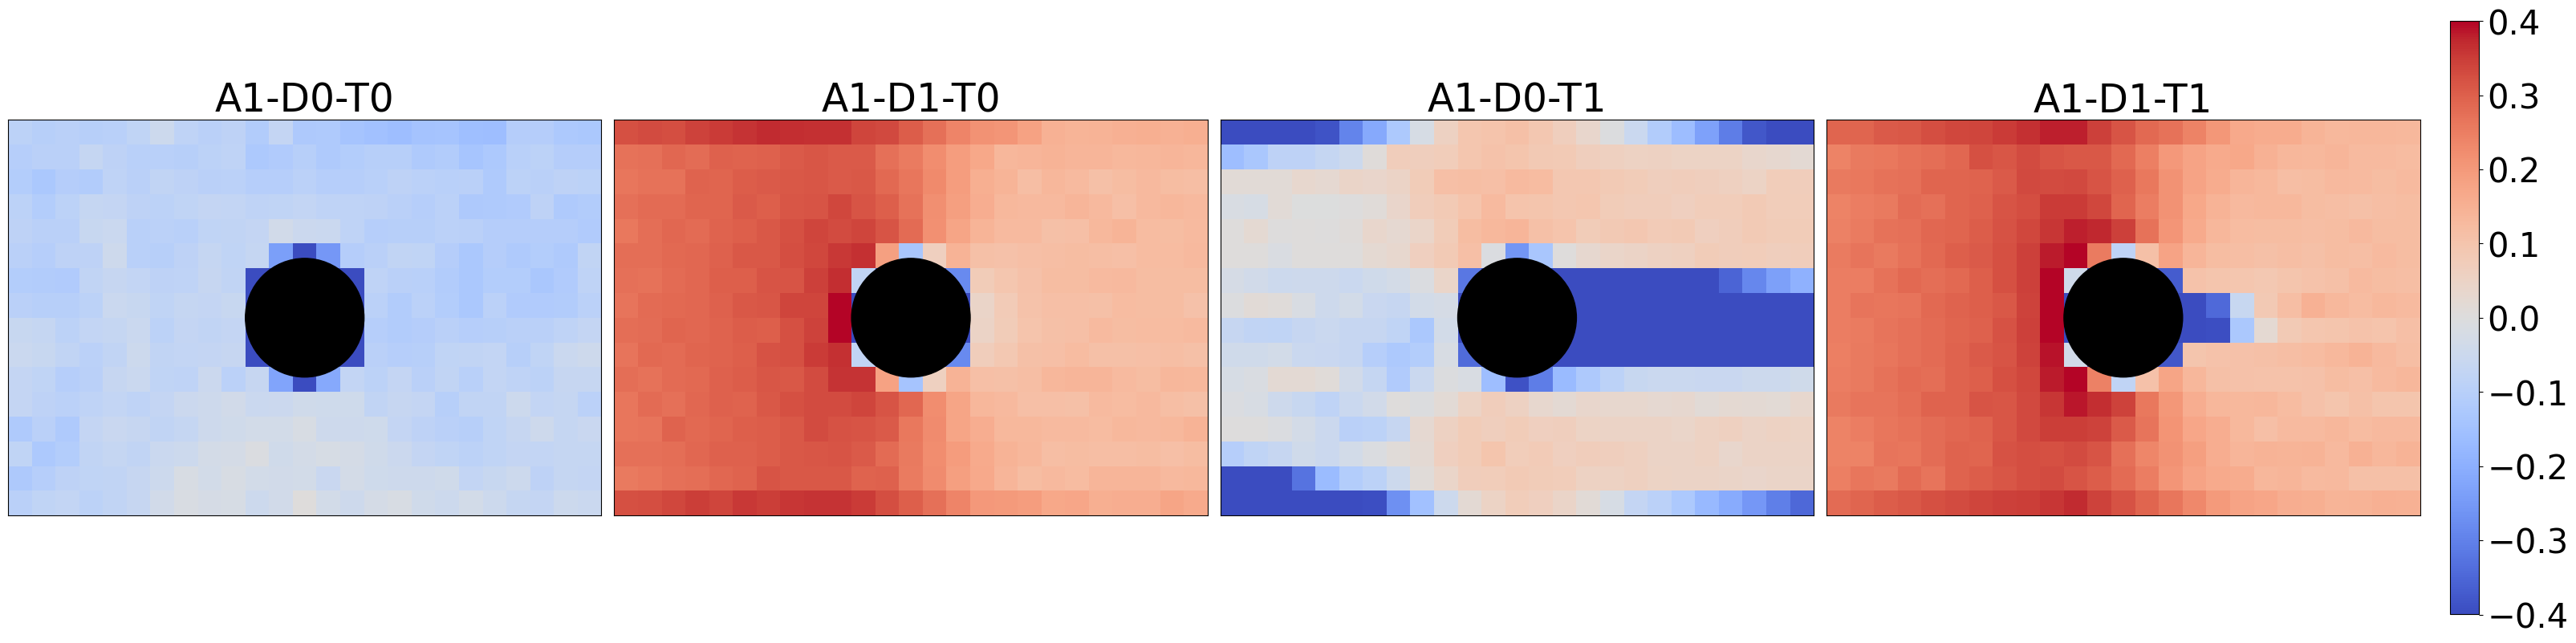
\includegraphics[width=\linewidth]{figuras/output_measurements/den_high_align.png}
    \caption{Campo da densidade relativa para os casos de alinhamento alto. A cor vermelha indica que os anéis estão comprimidos e a azul que existe espaço vazio entre os anéis.}
    \label{fig:output_rel_den_high_align}
\end{figure}

\FloatBarrier

\subsection{Phystem}
\paragraph{}
Para facilitar a reprodução dos dados aqui apresentados, bem como a exploração de casos semelhantes, mas com configurações diferentes, foi desenvolvido uma biblioteca de código aberto, chamada de \textit{Phystem}, que contém uma implementação do presente modelo em geometria de Stokes. 

O objetivo principal do \textit{Phystem} é prover uma plataforma onde sistemas físicos podem ser implementados e compartilhados com facilidade. Sua arquitetura consiste em um núcleo e diferentes módulos (as implementações dos sistemas físicos) que utilizam desse núcleo. O núcleo possui funcionalidades básicas fundamentais, como um sistema de auto-salvamento do sistema enquanto a simulação ocorre, funcionalidade extremamente importante em simulações que demoram dias ou semanas.

Atualmente apenas existe um único módulo, o módulo dos anéis ativos. Praticamente tudo é configurável em simulação dos anéis dentro do \textit{Phystem}: todos os parâmetros mencionados na descrição do modelo, as dimensões geométricas do canal, etc. Ao configurar uma simulação, é possível gerar um arquivo que contém todas as suas configurações, esse arquivo é ideal para compartilhar simulações e é possível iniciar uma simulação a partir dele.

No módulo dos anéis, também existe um sistema de coletores e calculadores de dados. Todas as medidas aqui apresentadas foram feitas utilizando esse sistema.

Por fim, de nada adianta uma ferramente sem documentação, então foi criado uma sítio dedicado a prover documentação sobre todos os sistemas presentes no \textit{Phystem}, instruções de instalação e exemplos ilustrativos\footnote{Documentação do \textit{Phystem}: \href{https://marcos1561.github.io/phystem/}{https://marcos1561.github.io/phystem/}}. A documentação dedicada ao módulo dos anéis ativos possui exemplos práticos de como configurar e rodar uma simulação, como utilizar o sistema de coletores, dentre outras informações importantes.

\section{Cronograma para o TCC 2}
\begin{itemize}
    \item (\textbf{5 Semanas}): Executar as simulações para os 4 casos restantes, em que o alinhamento é baixo, coletando as medidas de entrada e saída.
    \item (\textbf{5 Semanas}): Analisar e interpretar os dados coletados.
    \item (\textbf{5 Semanas}): Realizar comparação com experimentos utilizando o perfil de velocidades no mesmo espirito da tese de doutorado \cite{shourick_modelisation_2024}.
    \item (\textbf{5 Semanas}): Finalizar a monografia e preparar a defesa.
\end{itemize}

\bibliographystyle{unsrt}
\bibliography{tcc.bib}
%\bibliography{referencias}

\end{document}
